\documentclass[oneside]{mgr}

\usepackage{polski}
\usepackage[utf8]{inputenc}
\usepackage{amsmath}	
\usepackage{graphicx}
\graphicspath{ {./} }
\usepackage{amsfonts}
\usepackage{hyperref}
\usepackage{tabstackengine}
\usepackage{caption}
\usepackage{subfig}

\newcommand{\bb}{\textbf}



\title{Biometryczny system kontroli dostępu - przetwarzanie obrazów i przygotowanie danych dla sieci neuronowych}
\engtitle{Biometric Control Access System - image processing and preparing data for neural networks}
\author{Jędrzej Kozal}
\supervisor{dr  inż. Piotr Ciskowski}

\field{Automatyka i Robotyka (AIR)}
\specialisation{Technologie informacyjne w systemach automatyki (ART)}

\begin{document}
\bibliographystyle{plabbrv}

\maketitle

\linespread{1.5}

\chapter{Wstęp}
Celem pracy jest porównanie metod i algorytmów umożliwiających wykrycie twarzy na zdjęciu, oraz wyznaczenie wektora uczącego dla sieci neuronowej na podstawie wyznaczonego zdjęcia twarzy. Projekt ten jest częścią systemu biometrycznej kontroli dostępu. Za implementację sieci neuronowych oraz analizę algorytmów związanych z sieciami odpowiadał Filip Guzy. Za architekturę systemu, oraz komunikację pomiędzy komponentami odpowiadał Michał Leś. 

Celem całego projektu było skonstruowanie prostego systemu kontroli dostępu opartego na rozpoznawaniu twarzy. System ma określać czy na wykonanym zdjęciu występuje twarz. Ponadto przedmiotem pracy było wyznaczenie sposobu na ekstrakcję cech ze zdjęcia i przygotowanie wektora uczącego dla sieci. Zadaniem sieci neuronowej jest klasyfikacja czy danemu użytkownikowi przyznano wcześniej dostęp czy też nie.

System oryginalnie został zaprojektowany na mikrokomputer Rasbery Pi. W projekcie wykorzystano Rasbery Pi 3. Przy projektowaniu systemu fakt ten miał niebagatelne znaczenie, ze względu na ograniczone pokłady mocy obliczeniowej. Architekutra systemu została zaprojektowana w taki sposób, aby system można było z łatwością przenosić na inne platformy. 


\section{Omówienie zagadnienia}

\section{Omawiany komponent jako część większego systemu}

Jak wspomniano we wstępie komponent opisany w niniejszej pracy jest częścią większego systemu. W tej sekcji pracy przedstawiono założenia projektowe, zaprezentowano szerszy ogląd na cały system. Omówiono komponent z programistycznego punktu widzenia: omówiono wzorce projektowe, praktyki jakich przesztrzegano projektując komponent oraz uzasadniono wybór narzędzi.

\subsection{Wykorzystane wzorce projektowe}

W celu ułatwienia pracy współpracownikom w projekcie został utworzony wydzielony łatwo wymienialny komponent. W celu ułatwienia pracy badawczej komponent został podzielony na mniejsze elementy z wykorzystaniem obiektowych wzorców projektowych.
Do reprezentacji całego komponentu wybrano wzorzec fabryka. Zapewniono w ten sposób elastyczność użytkownikom klasy, ponieważ mogą oni zdecydować w jaki sposób współrzędne będące wynikiem działania algorytmów mają być przedstawione. Zapewniono klasę bazową do przechowywania współrzędnych, po której dziedziczą poszczególne reprezentacje, takie jak bezpośrednie przechowywanie danych w pamięci programu, czy zapis na pamięć nieulotną w postaci pliku z rozszerzeniem .npy z biblioteki numpy.
W celu zwiększenia elastyczności w obrębie komponentu do wyboru algorytmów dwukrotnie wykorzystano wzorzec strategia. Stworzono klasy bazowe do reprezentacji podstawowych własności algorytmu, które następnie implementowano w klasach pochodnych. Modyfikacja ta ułatwiła pracę badawczą i usystematyzowała strukturę projektu.

\subsection{Wykorzystane zasady i dobre praktyki programowania}

W trakcie realizacji projektu oprócz wykorzystania wzorców projektowych posługiwano się także dobrymi zasadami SOLID oraz clean code. Pozwalają one na zachowanie większego porządku oraz czytelności kodu. Dobra organizacja kodu oraz porządek ułatwiają rozwijanie projektu oraz systematyzują pracę. Nie zdecydowano się na wykorzystanie testów jednostkowych ze względu na dynamiczny charakter projektu. Definiowanie zachowań w testach jednostkowych jest kosztowne, a częste zmiany powodują że praca ta momentami byłaby zbędna.

\subsection{Wykorzystane biblioteki, narzędzia i zasoby}
Projekt systemu biometrycznej kontroli dostępu został zrealizowany całkowicie w języku programowania Python. Decyzja ta była podyktowana głównie znaczącą ilością gotowych bibliotek, które znacząco ułatwiają pracę. Wykorzystana została wersja języka 2.7.9, ponieważ biblioteki języka Python często wymagają wersji 2.7 lub wyższej. W omawianym komponencie wykorzystano biblioteki NumPy, SciPy, scikit-learn, openCV oraz Dlib. 
NumPy to biblioteka zawierająca wiele algorytmów do realizacji obliczeń numerycznych oraz implementację wielu matematycznych narzędzi związanych z algebrą liniową. Implementacja algorytmów macierzowych z NumPy cieszy się dużą popularnością, dlatego warto poświęcić czas na poznanie tej biblioteki, ponieważ stanowi ona fundament wielu innych projektów i bibliotek.
SciPy jest biblioteką wykorzystywaną do obliczeń naukowych i inżynierskich. Zawiera algorytmy umożliwiające przeprowadzane obliczeń w wielu dziedzinach, dlatego również jest wykorzystywana jako baza innych projektów.
Instalacja SciPy jest prerekwizytem do instlacji scikit-learn. Scikit-learn to biblioteka zawierająca wiele algorytmów z dziedziny machine learning oraz pattern recognition. Jest to kluczowa bilioteka w omawianym projekcie, ponieważ dostarcza najistatniejszych narzędzi. Jej zastosowanie znacznie ułatwiło pracę.
OpenCv stanowi poteżny zbiór narzędzi do analizy oraz przetwarzania obrazów. Rozpowszechniana w ramach licencji . Twórcy biblioteki skupiają się na działanie w czasie rzeczywistym i zapewniają wielordzeniowe przetwarzanie. Jest to znaczące ułatwienie biorąc pod uwagę podstawową platformę sprzętową, na której był realizowany projekt. 
Dlib jest biblioteką przewidzianą głównie dla języka C++, jednakże możliwe jest także wykorzystanie jest w Pythonie. Zawiera głównie algorytmu z dziedziny ML. W omawianym projekcie została wykorzystana do zbadania możliwości alternantywnych metod detekcji twarzy.

Wszystkie wymienione biblioteki są rozpowszechniane w ramach licencji new-BSD lub 3-clause BSD, co oznacza że wolno je wykorzystywać w celach akademickich lub komercyjnych. Zastosowanie bibliotek dostarczających zoptymalizowanych algorytmów znacznie ułatwiło i usystematyzowało pracę nad projektem.

Na początku pracy nad projektem podjęto próbę implementacji własnej wersji algorytmu PCA, aby lepiej zrozumieć i dokładnie prześledzić jego działanie. Algorytm ten działał poprawnie, ale względu na dużą złożoność obliczeniową zdecydowano się na korzystanie z wersji udostępnionej w bibliotece scikit-learn. W trakcie późniejszych prac nad systemem znaleziono informację na temat tego co powodowało tak wysoką złożoność obliczeniową oraz sposób na jej uniknięcie. Zagadnienie to zostało opisane w rozdziale Realizacja algorytmu.

Diagramy i rysunki wykonano z wykorzystaniem strony draw.io. Do wszystkich zapożyczonych obrazów zostały podane źródła.

Do przeprowadzenia badań jako bazy twarzy wykorzystano zbiór zdjęć dostępny w ramach biblioteki scikit-learn The Olivetti faces dataset. Posłużył on jako baza do wyznaczenia wartości własnych przestrzeni zdjęć twarzy.

\newpage

\chapter{Implementacja algorytmów – detekcja twarzy}

Pierwszym wymaganiem po zdolności do akwizycji obrazów jest określenie czy uzyskane zdjęcie przestawia twarz. W niniejszym rozdziale omówiono możliwe metody detekcji twarzy na dwuwymiarowym obrazie. Szczegółowo omówiono przyjęte rozwiązanie, oraz podano uzasadnienie dlaczego zostało ono wybrane.

\section{Kaskady Haara}
Alogrytm Kaskad Haara (lub detektor Viola-Jones) wykorzystuje serię cech do określenia czy na zdjęciu w określonym miejscu znajduje się szukany obiekt. Cecha jest tutaj rozumiana jako prostokąt podzielony na części. Pod każda z części dodawane są wartości pikseli, następnie wartości z obu obszarów są od siebie odejmowane. Pomysł ten przypomina falkę Haara, stąd nazwa algorytmu. Tak uzyskana wartość musi przekroczyć odpowiedni próg, który decyduje o tym czy w danym miejscu rozpoznano twarz. Jak podano w \cite{Kaskada Haara}, aby móc szybciej obliczać wartości pikseli pod odpowiednim obszarem wykorzystuje się obraz kumulacyjny (ang. integral image). Jest on zdefiniowany jako:

\begin{equation}
	ii(x,y) = \sum_{x' \leq x, y' \leq y} i(x',y')
\end{equation}

Funkcja ta przypomina dyskretną dystrybuantę dwuwymiarowej zmiennej losowej. Jej zastosowanie pozwala na obliczenie sumy jasności pod dowolnie wielkim obszarem, w dowolnym miejscu obrazu w stałym czasie.

\begin{figure}
\centering
	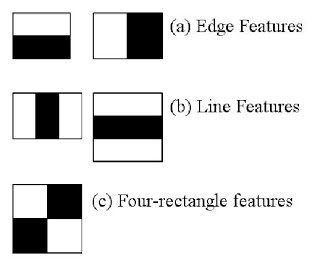
\includegraphics[width=0.50\textwidth,natwidth=610,natheight=642]{haar_features.jpg}\par\vspace{0.5cm}
\caption{Różne rodzaje cech. Od sumy wartości pikseli po czarnym obszarem jest odejmowana wartość sumy pikseli pod białym polem.}
Źródło: https://docs.opencv.org\/3.3.0\/d7\/d8b\/tutorial\_py\_face\_detection.html
	\label{fig:features}
\end{figure}

Nawet dla najmiejsznych obrazów można rozważać wiele cech. W celu ograniczenia ilości analizowanych cech wykorzystano alogrytm AdaBoost \cite{AdaBoost}. Alogrytm ten dysponując zbiorem uczącym oraz zbiorem słabych hipotez przydziela wagi hipotezom, oceniając ich skuteczność. Dodatkowo wagi otrzymują także przykłady ze zbioru uczącego. Każdorazowo kiedy dany przykład zostanie źle zaklasyfikowany, jego waga jest zwiększana. 


\begin{figure}
\centering
	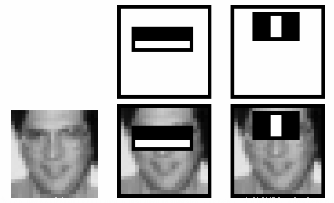
\includegraphics[width=0.50\textwidth,natwidth=610,natheight=642]{haar.png}\par\vspace{1cm}
\caption{Dwie cechy generujące najmniejszy błąd z wykorzystaniem AdaBoost.}
Źródło: https://docs.opencv.org\/3.3.0\/d7\/d8b\/tutorial\_py\_face\_detection.html
	\label{fig:best_features}
\end{figure}

Wykorzystanie AdaBoost pozwoliło na wybranie cech generujących najmniejszy błąd. Ilość użytych cech wpływa na jakość algorytmu, jednocześnie zwiększając czas potrzebny na obliczenia. Jak można zauważyć na \ref{fig:best_features} najlepsze cechy mają dość intuicyjną interpretację: spodziewamy się że obraz w okolicach oczu będzie ciemniejszy niż w okolicach policzków, oraz że środek nosa będzie jaśniejszy niż obszary po bokach.

Dysponując zbiorem chech można przystąpić do klasyfikacji obrazu. Odbywa się to kaskadowo. W pierwszym etapie wykorzystuje się klasyfikator złożony najczęściej z jednej lub dwóch cech. Klasyfikacja jest przperowadzana na całym obrazie, aby wykryć gdzie może znajdować się twarz. W kolejnych etapach ilość cech jest zwiększana (najczęściej wykładniczo). Jeśli w danym obszarze nie została wykrytwa twarz zostaje on pominięty w dalszych etapach. Pozwala to znacząco ograniczyć ilość wykonywanych operacji. Zaleca się aby w pierwszym etapie wykorzystawać cechę z wysokim współczynnikiem fałszywych negatywnych rezultatów (ang. false negative) - w tym przypadku obszarów zawierających twarz błędnie zaklasyfikowanych jako nie będących twarzą.

Kaskady Haara są szybkie, przez co chętnie wykorzystuje się je w zastoswaniach wymagającego przetwarzania obrazów w czasie rzeczywistym. Było to także motywacją przy wyborze tej metody w omawianym systemie. Rozwiązanie daje to zadowalające wyniki przy jednoczesnym szybkim działaniu. W rozważanym systemie kosztowność obliczeniowa musi być brana pod uwagę, biorąc pod uwagę, że oryginalna platforma sprzętowa na którą został przewidziany system to Rasbery Pi.

\section{Inne sposoby rozwiązanie problemu}

\begin{figure}
\centering
	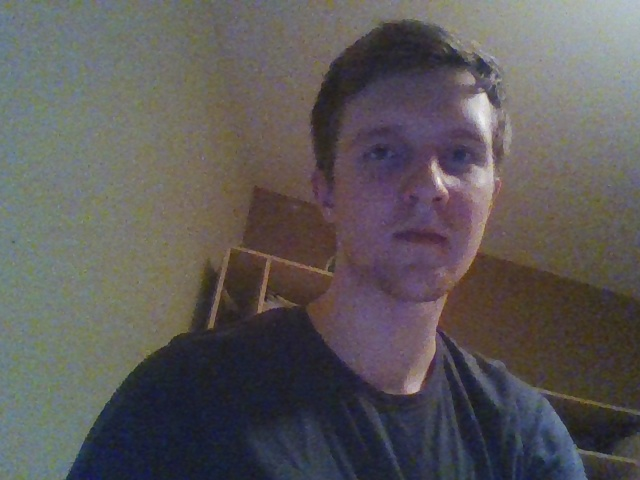
\includegraphics[width=0.40\textwidth,natwidth=310,natheight=642]{test.jpg}
	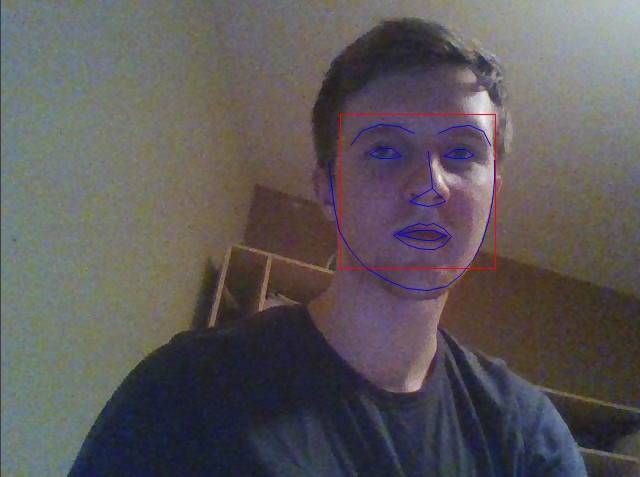
\includegraphics[width=0.40\textwidth,natwidth=310,natheight=642]{test_result.jpg}
\caption{Wykrywanie punktów charakterystycznych twarzy.}
Po lewo oryginalny obraz, po prawo obraz z zaczaczonym rezultatami detekcji. Do detekcji wykrozystano 68 cech.
	\label{fig:face_landmark_detect}
\end{figure}

Do całego problemu można zastosować inne podejscie polegające na szukaniu charakterystycznych punktów twarzy. W pracy \cite{Landmark face detector} wykorzystano boosting drzewa gradientu do stworzenia kaskady regresorów. Dysponując zbiorem uczącym zawierającym zdjęcia twarzy oraz współrzędne punktów charakterystycznych można wyznaczyć kaskadę regresorów liniowych. Zakładamy że estymowany kształt punktów charakterystycznych dowolnej twarzy może być wyrażony jako kombinacja liniowa kształtu punktów charakterystycznych z odpowiednio dużego zbioru uczącego. Każdy regresor to drzewo decyzyjne, które w liściach przechowuje wektor, który powinien zostać dodany do aktualnej ekstymacji punktów charakterystycznych (zbiór współrzędnych x i y które powinny być kolejno dodane do każdej współrzędnej). W pierwszym kroku jako estymacja jest wykorzystywany średni kształt z bazy zdjęć uczących. Następnie każdy regresor delikatnie poprawnia estymację, przesuwając punkty w odpowiednią stronę. Na rys. \ref{fig:face_landmark_detect} przedstawiono efekty detekcji twarzy z wykorzystaniem implelmetancji z biblioteki Dlib.

Omawiane rozwiązanie umożliwia całkowicie inne podejście do problemu ekstrakcji cech. Mając wyestymowane charakterystyczne punkty twarzy, oraz mierząc odległości między poszczególnymi punktami można przygotować wektor uczący mający bardzo fizyczne interpretację. Dodając informację na temat koloru oczy czy skóry, można skonstruować zupełnie inne wektory cech niż proponowany w tej pracy. 

\newpage
 
\chapter{Implementacja algorytmów – ekstrakcja cech}

Ninjeszy rozdział traktuje o algorytmach umożliwiających ekstrakcję cech twarzy ze zdjęcia. Dysponując zdjęciem twarzy należy zaproponować sposób utworzenia wektora, będącego reprezentatywnym odzwierciedleniem ilościowych cech ze zdjęcia i jednocześnie umożliwi sieci neuronnowej dokonanie klasyfikacji. Zadanie to jest bardzo abstrakcyjne, zależy od wielu czynników i trudno jest określić rezultaty.

W rozdziale tym skupiono się głównie nad podejściem polegającym na zastosowaniem algorytmów redukcji wymiarowości, takich jak PCA czy SVD. Jest to dość popularne rozwiązanie i w przypadku PCA można uzyskać wyniki mające wizualną interpretację, co jest bardzo pomocne przy pracy nad tego typu problemem.

Obraz po wykryciu twarzy jest obcniany do kwadratu, na którym wykryto twarz, następinie obraz jest obcinany do rozmiaru 64 $\times$ 64, w celu ujednolicenia rozmiarów przetwarzanych obrazów oraz zwiększenia szybkości przetwarzania.
 
\section{Principle Components Analysis}

Principle Components Analysis (PCA) jest algorytmem redukcji wymiarowości danych. Mając określony zbiór obserwacji, będący reprezentatywną reprezentacją próbą analizowanej przestrzeni należy wyznaczyć zbiór wektorów bazowych, tak aby wariancja danych z zbioru obserwacji względem nowo wyznaczownych wektorów bazowych była jak najwyższa.

\subsection{Wstęp matematyczny}

Przedstawione tutaj wyprowadzenie jest podawane za Pattern recognition and machine learning.

Zakładamy że dany jest zbiór $D$-wymiarowych wektorów obserwacji: $\bb{x}_n , n \in 1,...,N $. Celem jest znalezienie nowej $M$-wymiarowej bazy ($M < D$), takiej że wariancja zbioru wektorów $\bb{x}_n$ po zrzutowaniu na nową bazę jest największa. W celu pokazania procesu i rozumowania przyjmijmy że szukamy jednego wektora $\bb{u}_1$. Wektor ten, ponieważ ma stanowić bazę musi być D-wymiarowy. Dodatkowo przyjmiejemy że wektor $\bb{u}_1$ jest jednostkowy, co zapiszemy w postaci warunku:
\begin{equation} \label{eq:wektor_jednostkowy}
	\bb{u}_1^{T}\bb{u}_1 = 1
\end{equation}

Rzut wektora \bb{x} na kierunek wyznaczany przez wektor \bb{u} jest dany przez: $u^{T}x$. Fakt ten ma proste uzasadnienie geometryczne:
\begin{align*}	
	\bb{u}^{T} \bb{x} &= \bb{u} \circ \bb{x} \\
		   & = ||\bb{u}|| ||\bb{x}|| cos \angle (\bb{u}, \bb{x}) \index{1} \\
		   &= ||\bb{x}|| cos \angle (\bb{u}, \bb{x}) \index{1} && \text{(\ref{eq:wektor_jednostkowy})}
\end{align*}

Przyjmimy średnią jako estymator wartości oczekiwanej:
\begin{equation}	\overline{\bb{x}} = \frac{1}{N} \sum_{n=1}^{N} \bb{x}_n \end{equation}

Wariancja zmiennej losowej $X$ jest dana przez:
\begin{align*}	\notag
	var[X]  &= \mathbb{E}[(X - \mathbb{E}[X])^2] \\
			&= \mathbb{E}[X^2] - \mathbb{E}[X]^2
\end{align*}

Wariancja jest miarą rozrzutu wartości zmiennej losowej. Im większe różnice między wartościami przyjmowanymi przez zmienną losową, tym większa jest wariancja.

Estymator wariancji dla próby losowej $x_n$:
\begin{equation}	\notag
	s^2 = \frac{1}{N} \sum_{n=1}^{N}(x_n - \overline{x})
\end{equation}

Kowariancja między dwoma zmiennymi losowymi jest dana wzorem:
\begin{align}	
	cov[X,Y] &= \mathbb{E}[(X - \mathbb{E}[X])(Y - \mathbb{E}[Y])]  \label{eq:cov} \\ 
			 &= \mathbb{E}[XY] - \mathbb{E}[X]\mathbb{E}[Y] \nonumber
\end{align}

Wzór ten można uogólnić dla wektorów losowych:
\begin{align*}
	cov[\textbf{X}, \bb{Y}] &= \mathbb{E}[(\bb{X} - \mathbb{E}[\bb{X}])(\bb{Y}^T - \mathbb{E}[\bb{Y}^T])] \\
							&= \mathbb{E}[\bb{X}\bb{Y}^T] - \mathbb{E}[\bb{X}]\mathbb{E}[\bb{Y}^T]
\end{align*}

Definiujemy macierz kowariancji S dla zbioru obserwacji $\bb{x}_n$:
\begin{equation}
	S = \frac{1}{N} \sum_{n=1}^{N} (\bb{x}_n - \overline{\bb{x}})(\bb{x}_n - \overline{\bb{x}})^T
\end{equation}

Jak łatwo zauważyć w powższym wzorze wartości oczekiwane zostały zastąpione średnimi, ponieważ nie dysponujemy rozkładami zmiennnych losowych, tylko zbiorem obserwacji.

Definiujemy wariancję zbioru obserwacji względem wektora $u_1$:
\begin{equation}
	s^2 = \frac{1}{N} \sum_{n=1}^{N}(\bb{u}_1^T \bb{x}_n - \bb{u}_1^T\overline{\bb{x}})^2 = \bb{u}_1^T S \bb{u}_1
\end{equation}

Chcąc maksymalizować wariancję $s^2$ musimy pamiętać o warunku $\ref{eq:wektor_jednostkowy}$. Otrzymujemy więc probelm optymalizacji polegający na znalezieniu maksimum warunkowego funkcji $f(\bb{u}_1)$ z ograniczniem $g(\bb{u}_1)$:
\begin{align*}
	f(\bb{u}_1) &= \bb{u}_1^T S \bb{u}_1 \\
	g(\bb{u}_1) &= 1 - \bb{u}_1^T \bb{u}_1 = 0
\end{align*}

Jest to problem, który można łatwo rozwiązać z wykorzystaniem mnożników Lagrange'a. W analizowanym przypadku Lagrangian przyjmuje postać:
\begin{align*}
	\mathcal{L}(\bb{u}_1, \lambda) &= f(\bb{u}_1) - \lambda g(\bb{u}_1) \\
				&= \bb{u}_1^T S \bb{u}_1 - \lambda(1 - \bb{u}_1^T \bb{u}_1)
\end{align*}

Różniczkując względem $\bb{u}_1$ oraz $\lambda$ oraz przyrównując do zera uzyskujemy układ równań:
\begin{align}
\begin{cases}
	\nabla_{\bb{u}_1} \mathcal{L} (\bb{u}_1, \lambda) &= \nabla_{\bb{u}_1} \bb{u}_1^T S \bb{u}_1 - \nabla_{\bb{u}_1} \lambda \bb{u}_1^T \bb{u}_1 = 0 \\
	\frac{\partial}{\partial \lambda} \mathcal{L} (\bb{u}_1, \lambda) &= 1 - \bb{u}_1^T \bb{u}_1 = 0
\end{cases}
\end{align}

Zajmijmy się pierwszym równaniem z $(6)$. Odjemnik można bardzo łatwo uprościć:
\begin{equation}
	\nabla_{\bb{u}_1} \lambda \bb{u}_1^T \bb{u}_1 = \lambda \nabla_{\bb{u}_1} 
		(u_{1_1}^2 + u_{1_2}^2 + ... + u_{1_D}^2)
	 	= 2 \lambda \bb{u}_1
\end{equation}

Odjemna wymaga wiecej przekształceń:
\begin{align}
	\nabla_{\bb{u}_1} \bb{u}_1^T S \bb{u}_1 
	&= \nabla_{\bb{u}_1} 
	\left( \begin{array}{llll} u_{1_1} & u_{1_2} & ... & u_{1_D} \end{array} \right)
	\begin{pmatrix}
         s_{1_1} u_{1_1} + s_{1_2} u_{1_2} + ... + s_{1_D} u_{1_D}  \\
		 s_{2_1} u_{1_1} + s_{2_2} u_{1_2} + ... + s_{2_D} u_{1_D} && \\
		 \vdots     \\
		 s_{D_1} u_{1_1} + s_{D_2} u_{1_2} + ... + s_{D_D} u_{1_D} && \\
    \end{pmatrix} \\
    &= \nabla_{\bb{u}_1} [u_{1_1} (s_{1_1} u_{1_1} + s_{1_2} u_{1_2} + ... + s_{1_D} u_{1_D})  \\
    				&+ u_{1_2} (s_{2_1} u_{1_1} + s_{2_2} u_{1_2} + ... + s_{2_D} u_{1_D}) \nonumber \\
    				&+ ... + u_{1_D} (s_{D_1} u_{1_1} + s_{D_2} u_{1_2} + ... + s_{D_D} u_{1_D})] \nonumber \\
    &= \begin{pmatrix}
    	2 s_{1_1} u_{1_1} + 2 s_{1_2} u_{1_2} + ... + 2 s_{1_D} u_{1_D}  \\
    	2 s_{2_1} u_{1_1} + 2 s_{2_2} u_{1_2} + ... + 2 s_{2_D} u_{1_D}  \\
    	\vdots     \\
	    2 s_{D_1} u_{1_1} + 2 s_{D_2} u_{1_2} + ... + 2 s_{D_D} u_{1_D}
    \end{pmatrix} \\
    &= 2 S \bb{u}_1
\end{align}

W przejściu między $(9)$ a $(10)$ korzystamy z faktu że macierz S (macierz kowariancji) jest symetryczna.

Wracając do $(6)$:
\begin{align}
	2 S \bb{u}_1 &- 2 \lambda \bb{u}_1 = 0	\nonumber \\
	S \bb{u}_1 &= \lambda \bb{u}_1 
\end{align}

Jest równanie na wartości własne macierzy S, więc $u_1$ musi być wektorem własnym macierzy S, $\lambda$ wartością własną macierzy S.

Mnożąc $(11)$ lewostronnie przez $u_1^T$ otrzymujemy:
\begin{equation}
	\bb{u}_1^T S \bb{u}_1 = \lambda
\end{equation}

Lewa część $(13)$ to wariancja, która ma być maksymalizowana. Aby uzyskać jak największą wariancję zbioru obserwacji po zrzutowaniu na kierunek wyznaczany przez $\bb{u}_1$ należy wybrać największą wartość własną macierzy S. Odpowiadający jej wektor własny jest szukanym wektorem $\bb{u}_1$. Dla kolejnych wektorów $\bb{u}$ należy znaleźć kolejne największe wartości własne i wektory własne.

\subsection{Realizacja algorytmu} 
Korzystając z PCA można zniejszyć wymiarowość danych w taki sposób aby zachować najwięcej informacji. Działanie algorytmu można zasadniczo podzielić na dwa etapy. Pierwszy to uzyskanie bazy wektorów, która zostanie wykorzystana w drugim etapie do uzyksania nowej reprezentacji wektorów z oryginalnej przestrzeni.

W pierwszym etapie należy obliczyć wartości własne macierzy kowariancji, jak to zostało pokazane w poprzednim dziale. Przyjmijmy że dysponujemy macierzą pomiarów:
\begin{align}
	X_{D \times N} = 
	\left( \begin{array}{llll}
		\bb{x}_1 & \bb{x}_2 & \ldots & \bb{x}_N
	\end{array} \right)	
	=
	\left( \begin{array}{llll}
		x_{1_1} & x_{1_2} & \ldots & x_{1_N} \\
		x_{2_1} & x_{2_2} & \ldots & x_{2_N} \\
		\vdots  & \vdots  & \ddots & \vdots  \\
		x_{D_1} & x_{D_2} & \ldots & x_{D_N}
	\end{array} \right)
\end{align}

Zdefinujmy macierz A, powstałą w wyniku odjęcia od każdego wiersza średniej:
\begin{equation}
	A_{D \times N} = 
	\left( \begin{array}{llll}
	\bb{x}_1 - \overline{\bb{x}} & \bb{x}_2 - \overline{\bb{x}} & \ldots & \bb{x}_N - \overline{\bb{x}}
	\end{array} \right)
\end{equation}


Dysponując macierzą A, można zapisać S w postaci:
\begin{equation}
	S_{D \times D} = \frac{1}{N} A A^T
\end{equation}

Co jest całkowcie zgodnie z definicją \ref{eq:cov}. Kolejnym krokiem będzie wyznacznie wektorów i wartości własnych, posortowanie wektorów własnych według nierosnącej wartości własnych oraz wybranie M wektorów wałasnych. 

Należy zwrócić uwagę na wymiar macierzy S. Przypomnijmy że D to wymiar wektora pomiarowego, co w przypadku zdjęć oznacza wartość każdego piksela przeniesiona kolejno do elementów wektora. W pracy tej zdjęcia przed podaniem na wejście algorytmu ekstrakcji cech były konwertowane do skali szarości i obcinane do rozmiaru 64 $\times$ 64 pikseli, co oznacza że wektor pomiarowy zawierał 4096 współrzędnych. Biorąc pod uwagę złożoność obliczeniową alogrytmów szukania wektorów własnych może to powodować problemy z wydajnością. Można temu zapobiec poprzez zamianę miejscami macierze $A$ i $A^T$ w iloczynie. Obliczając wartości własne macierzy $A^T A$ musimy wrócić do $D$-wymiarowości przestrzeni, co jest możliwe z wykorzystaniem następującej własności:
\begin{equation}
	u_i = A v_i
\end{equation}

Gdzie $v_i$ oznacza wartość własną macierzy $A^T A$. Poprzez zamianę miejscami macierzy $A$ i $A^T$ zyskujemy inny wymiar macierzy. Iloczyn ma teraz rozmiar NxN. Przypomnijmy że N to liczność zbioru obserwacji. Zazwyczaj N jest znacznie niższe od D, co może przyśpieszyć obliczenia. Korzystając z tego uproszczenia należy pamiętać że zostaje nałożone ogranicznie co wielkości M. Jako że zostają obliczone wektory własne macierzy o rozmiarze NxN, może ich być co najwyżej N. Oznacza że ilość wymiarów danych po redukcji nie może przekraczać ilość danych ze zbioru obserwacji ($M < N$). Ogranicznie to nie jest zbyt dotkliwe, gdy dysponujemy odpowiednio wielkim zbiorem testowym. W przypadku tej pracy dostępność danych stanowiących podstawę nie stanowiła problemu.

Po konwersji do oryginalnej wymiarowści dysponujemy bazą $M$ wektorów $D$-wymiarowych. Zbiór $M$ wektorów jest nazywany wartościami własnymi i zostanie wykorzystany w drugim etapie. Dla uproszczenia wektory własne zostaną włączone do jednej macierzy:
\begin{equation}
	U = 
	\left( \begin{array}{l}
		\bb{u}_1 \\
		\bb{u}_2 \\
		\vdots	 \\
		\bb{u}_M
	\end{array} \right)
\end{equation}
W pewnym sensie wyznacza on reguły przy pomocy których konwertujemy wektory $D$-wymiarowe na $M$-wymiarowe.

Drugim etapem działania algorytmu jest redukcja wymiarowości wektora $\bb{w}$ spoza zbioru obserwacji. Obrazowo można powiedzieć że na podstawie nowego zdjęcia, niewykorzystanego w poprzednim etapie chcemy uzyskać reprezentujący je wektor liczb, w przestrzeni o niższym wymiarze. Odbywa się to zasadniczo w dwóch bardzo prostych krokach: Pierwszym jest odjęcie od nowego wektora średniej. Drugim jest rzutowanie różnicy $\bb{w} - \overline{\bb{x}}$ na wcześniej uzyskane wartości własne. Uzyskanie współrzędnych w $M$-wymiarowej przestrzeni wektora $w$ można więc zapisać jako:
\begin{equation}
	U ( \bb{w} - \overline{\bb{x}} ) 
\end{equation}

Jak łatwo można zauważyć $\overline{\bb{x}}$ oraz $U$ zależą bezpośrednio od zbioru obserwacji jakim dysponujemy na początku. Dobranie zbioru reprezentatywnego dla danej przestrzeni jest kluczowe. Pierwszy etap działania algorytmu polegający na generacji wektorów własnych definiuje przekształcenie. Drugi etap działania pozwala na redukcję wymiarowości dowolnego $D$-wymiarowego wektora zgodnie z regułami ustalonymi w pierwszym kroku.

\subsection{Interpretacja}
Przyjrzyjmy się przez moment co tak na prawdę zyskujemy w wyniku działania algorytmu PCA. Przez odjęcie średniej przesuwamy środek nowopowstałego układu współrzędnych do punktu gdzie znajdowała się średnia zbioru obserwacji. Dodatkowo po odjęciu średniej wektor reprezentuje jedynie różnicę miedzy średnią (środkiem nowego układu współrzędnych), a punktem końcowym. Jest więc reprezentacją unikatowych cech w zbiorze obserwacji. Wybranie wektorów własnych, będących osiami - kierunkami z największą wariancją powoduje że odrzucając część bazy wektorów tracimy tak mało wektórów jak to jest tylko możliwe. W celach badawczych można wrócić do oryginalnej przestrzeni, aby porównać błąd przybliżenia oraz przeanalizować jak bardzo reprezentatyne są uzyskane wyniki. W przypadku zdjęć możliwa jest wręcz wizualne porównanie jak bardzo oryginalne zdjęcie i zdjęcie odtworzone po redukcji wymiarowości są podobne do siebie. Rekonstrukcja odbywam się w następujący sposób:
\begin{equation}
	v = \overline{x} + \sum_{n=1}^{M}u_n
\end{equation}

\begin{figure}
\centering
	\parbox{2cm}{
		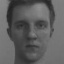
\includegraphics[width=2cm]{face_1.jpg}
		}
		\qquad
		\begin{minipage}{2cm}
			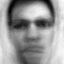
\includegraphics[width=2cm]{100.jpg}
		\end{minipage}
		\begin{minipage}{2cm}
			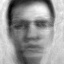
\includegraphics[width=2cm]{200.jpg}
		\end{minipage}
		\begin{minipage}{2cm}
			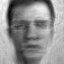
\includegraphics[width=2cm]{300.jpg}
		\end{minipage}
		\begin{minipage}{2cm}
			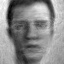
\includegraphics[width=2cm]{400.jpg}
		\end{minipage}
	\caption{Porównanie rekonstrukcji twarzy na postawie różnej liczby wykorzystanych składowych.} 
	Po lewej oryginalne zdjęcie, potem kolejno rekonstrukcja z wykorzystaniem 100, 200, 300 i 400 składowych.
	\label{fig:rekonstrukcja}
\end{figure}

Jak widać na rys. \ref{fig:rekonstrukcja} wraz ze zwiększeniem się ilości składowych jakość rekosntrukcji zdjęcia się polepsza. Użycie większej ilości składowych nie ma sensu, co można zaobserwować w wyglądzie rekonstrukcji z wykorzystanie 300 i 400 składowych. PCA jest bardzo lubianą metodą, ponieważ jest bardzo intuicyjna oraz pozwala na wizualne sprawdzenie własnych rezultatów.

W omawianym zagadnieniu wektory własne zyskały specjalną nazwę eigenfaces (twarze własne). Można zobaczyć jak wyglądają aplikując technikę odtwarzania zdjęcia na podstawie współrzędnych z przestrni o zredukowanej wymiarowości. Efekty zostały zaprezentowane na rys. \ref{fig:eigenfaces}. 

Jak można łatwo zaobserwować wektory 0-4 zawierają najbardziej istotne zmiany pomiędzy poszczególnymi obrazami ze zbioru obserwacji. Wektora 392-396 przypominają losowy szum i niosą informację o szczegółach twarzy. Można zauważyć że pominięcie składowych z niższą wartością własną powoduje mniejszą utratę informacji.

\subsection{PCA jako samodzielny system rozpoznawania twarzy}
Principle komponents analysis powoduje przeniesienie zdjęcia mającego wizualną reprezentację na abstrakcyjny wektor liczb. Umożliwia to skontruowanie klasyfikatora z wykorzystaniem algorytmów umożliwiających klasyfikację. Jest to zagadnienie dobrze znane w dziedzinie Pattern Recognition (rozpoznawania wzorców) i opracowano wiele rozwiązań tego problemu. Zastosowanie algorytmów typu k-NN (k Nearest Neighbour - k najbliższych sąsiadów) lub NM (Nearest Mean - najbliższy średnia) umożliwia zaklasyfikowanie danego algorytmu do jednej z grup. Jest to możliwie dzięki wykorzystaniu reprezentacji zdjęcia jako wektora liczb. Oba algorytmy dysponują zbiorem uczącym, który opisuje dane grupy do których może zostać klasyfikowany dany wzorzec. 
W przypadku NM dla każdej z grup obliczana jest średnia wektorów, następnie obliczana jest odległość między wektorem podlegającym klasyfikacji, a średnimi zbiorów. Wektor zostaje zaklasyfikowany do zbioru, którego średnia jest w najmniejszej odległości od wektora. 
W przypadku algorytmu k-NN odległość jest obliczana pomiędzy wszystkimi wektorami ze zbioru uczącego. Następnie zostaje wybrane k najbliższych sąsiadów. Zbiór, którego najwięcej przedstawicieli zostało wybranch wygrywa. Dla przypadku dychotomii jeżeli k jest nieparzyste możliwa jest jednoznaczna klasyfikacja. Gdy ilość zbiorów do których można zaklasyfikować obraz jest większa od dwóch możliwe jest wystąpienie wypadku w którym nie można jednoznacznie zaklasyfikować obiekt. 
W przypadku systemu kontroli dostępu może być rozsądne wprowadzenie maksymalnej odległości między średnią lub najbliższym sąsiadem a klasyfikowanym wektorem przy której może następić klasyfikacja. Powyżej tej odległości obraz nie powinien być zaklasyfikowany do którejkolwiek z grup. 
Dodatkowo warto zwrócić uwagę na brak kontroli PCA nad przetwarzanymi danymi. Jest to metoda statystyczna, na jej wejście można podać zdjęcie myszy lub samochodu, które zostanie przetworzone. Nie wiadomo jakie współrzędne można uzyskać, dzięki takiej operacji. System rozpoznawania twarzy powinien więc odrzucić takie zdjęcie na etapie wykrywania pozycji twarzy.

\section{Inne podejścia do problemu redukcji wymiarowości}


\newpage

\chapter{Zabezpieczenie przed możliwością oszukania systemu}

W trakcie realizacji projektu specjalnościowego podjęto próbę zadresowania kwesti oszukania całego systemu poprzez przedstawianie systemowi zdjęć ludzi, którym wcześniej przyznano prawo dostępu. Jest to realne zagrorzenie, z którym twórcy systemów biometrycznych muszą się mierzyć. Dobrym przykładem może być tutaj system FaceID w IphoneX firmy Apple. Twórcy systemu zapewniali że nie da go się oszukać poprzez wykonanie masek 3d imitujących twarz człowieka. 9 listopada 2017 roku ekseprci z firmy Bkav oświadczyli że udało im się złamać zabezpieczenia poprzez wykonanie specjalnej maski, wykorzystując drukarkę 3D, silikonowe elementy, wydruki 2D, oraz materiał imitujący skórę \cite{FaceID hacked}. Dodatkowo system FaceID okazał się nie być odporny na podobieństwo występujące między bliźniakami jednojajowymi. Bezpieczeństwo systemów biometrycznych jest więc bardzo ważną kwestią i podjęto próbę zbadania tych zagadnień.

\section{Przyjęta metodyka}
Zbadano możliwości jakie daje ekstrakcja głębi z wykorzystaniem dwóch kamer. W obecnym projekcie systemu zintegrowanie systemu ekstrakcji głębi byłoby trudne, ponieważ w projekcie wykorzystywana jest kamera Ruberby Pi, podłączona przez port CSI, a mikrokomputery Rasbry Pi posiadają tylko jeden port CSI. Do badań wykorzystano dwie kamerki internetowo Creative VF0770. Do ekstrakcji głębi wykorzystano funkcje biblioteki OpenCV. Celem było uzyskanie mapy punktów w 3D, które następnie miały być aproksymowane płaszczyzną. Następnie należało wyznaczyć błąd aproksymacji, oraz próg, od którego mapa punktów miała być uznawana za płaską.

\section{Podstawy teoretyczne}

Przed przedstawieniem wyników omówiono przyjęte założenia teoretyczne. W nimniejszej sekcji zostały omówione takie koncepcje jak pinhole camera model, model zniekształceń w biblitece OpenCv, podstawowe założenia geometrii epipolarnej oraz wyznaczanie mapy głębokości na podstawie dysparycji.

\subsubsection{Model kamery}
Przed przystąpieniem do ekstrakcji głębi należy ustalić model działania pojedyńczej kamery oraz zrozumieć jakie zakłócenia obrazu występują.

\begin{figure}
\centering
	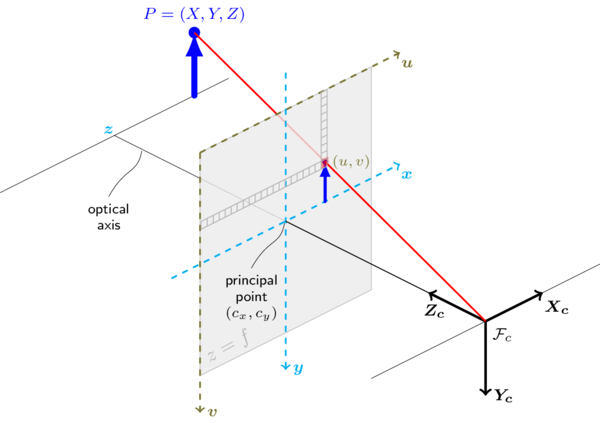
\includegraphics[width=0.90\textwidth]{pinhole_camera_model.png}\par\vspace{1cm}
\caption{Scena przy przyjętym modelu kamery.}
Źródło: https://docs.opencv.org/2.4/modules/calib3d/doc/camera\_calibration\_and\_3d\_reconstruction.html
	\label{fig:camera_model}
\end{figure}

Najczęściej rozpowszechnionym modelem jest tzw. pinhole camera model. W modelu tym kamera przekształca piksele z globalnego układu współrzędnych do układu współrzednych na płaszczyźnie, na którą są rzutowane punkty. Przekształcenie to można wyrazić wzorem:

\begin{equation}
	Z
	\left( \begin{array}{l}
		u \\
		v 
	\end{array} \right) 
	= K (R \quad T) 
	\left( \begin{array}{l}
		X \\	Y \\	Z \\	1
	\end{array} \right) 
\end{equation}

W powyższym równaniu $X, Y$ oraz $Z$ to współrzędne punktu w zewnętrznym układzie współrzędnych.
$u$ i $v$ to współrzędne w układzie kamery.
Macierz R i wektor T to macierz rotacji i wektor translacji opisujące orientację i położenie kamery względem zewnętrznego układu współrzędnych. Zaliczaję się one do parametrów zewnętrznych, ponieważ nie zależą od samej kamery, ale od jej położenia i oreintacji. Parametry te opisują transformację punktu z globalnego układu współrzędnych do układu współrzędnych kamery. 

\begin{align*}
	\left( \begin{array}{l} x \\ y \\ z \end{array} \right) =
	(R \quad T)
	\left( \begin{array}{l}
		X \\	Y \\	Z \\	1
	\end{array} \right) 
\end{align*}

Gdzie $x, y, z$ to współrzędne punktu P w układzie kamery.


\begin{figure}
\centering
	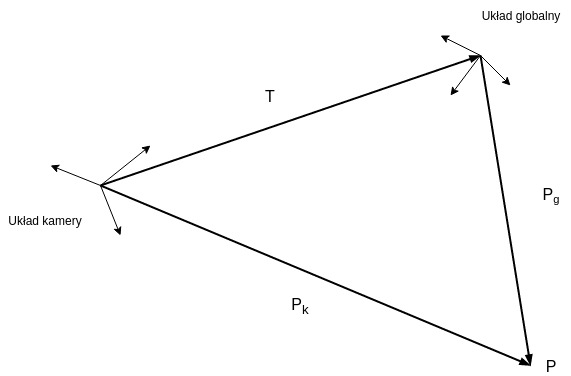
\includegraphics[width=0.90\textwidth]{pinhole.jpg}\par\vspace{1cm}
\caption{Ilustracja zależności między układami współrzędnymi a punktem.}
	\label{fig:camera_coordinate_systems}
\end{figure}

Warto zwrócić uwagę że wektor $T$ zawiera położenie globalnego układu współrzędnych względem układu współrzędnych kamery, a nie odwrotnie. Fakt ten może wydawać nieco nieintuicyjny, ale można go łatwo zilustrować. Z \ref{fig:camera_coordinate_systems} wynika jednoznacznie że $P_k = T + P_g$. Oczywiście należy uwzględnić wzajmeną orientację układów, co zapewnia macierz R.

Macierz K jest zawiera parametry wewnętrzne kamery i jest definiowana jako:
\begin{equation}
	K = \left( \begin{array}{lll}
		f & 0 & c_x \\
		0 & f & c_y \\
		0 & 0 & 1
	\end{array} \right)
\end{equation}

Gdzie $f$ to długość ogniskowej, $c_x, c_y$ jest punktem w którym oś optyczna przecina się płaszczyzną obrazu (ang. principal point), zwykle znajdujący się w środku obrazu.

Kokrzystając z wcześniejszych równań można zapisać:

\begin{align*}
	u = f \frac{x}{z} + c_x \\
	v = f \frac{y}{z} + c_y
\end{align*}

\begin{figure}
\centering
	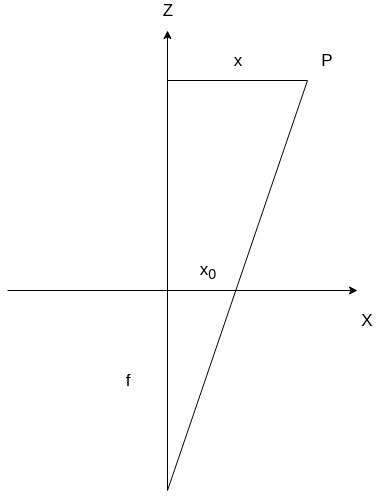
\includegraphics[width=0.50\textwidth]{rzutowanie.jpg}\par\vspace{1cm}
\caption{Rzut z góry na scenę.}
	\label{fig:projection_up}
\end{figure}

Na rys \ref{fig:projection_up} można zauważyć że równania te mają proste uzasadnienie geometryczne. Z twierdzenia Talesa otrzymujemy: 
$\frac{x_0}{f} = \frac{x}{z}$. Wartość $u$ możemy uzskać poprzez dodanie do $x_0$ z poprzedniego równania $c_x$. Dla y rozumowanie jest analogiczne.



\begin{figure}
\centering
	\parbox{2cm}{
		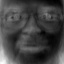
\includegraphics[width=2cm]{0.jpg}
		}
	\begin{minipage}{2cm}
		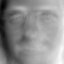
\includegraphics[width=2cm]{1.jpg}
	\end{minipage}
	\begin{minipage}{2cm}
		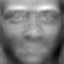
\includegraphics[width=2cm]{2.jpg}
	\end{minipage}
	\begin{minipage}{2cm}
		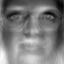
\includegraphics[width=2cm]{3.jpg}
	\end{minipage}
	\begin{minipage}{2cm}
		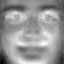
\includegraphics[width=2cm]{4.jpg}
	\end{minipage}\\
	
	\begin{minipage}{2cm}
		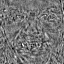
\includegraphics[width=2cm]{392.jpg}
	\end{minipage}
	\begin{minipage}{2cm}
		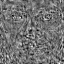
\includegraphics[width=2cm]{393.jpg}
	\end{minipage}
	\begin{minipage}{2cm}
		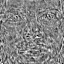
\includegraphics[width=2cm]{394.jpg}
	\end{minipage}
	\begin{minipage}{2cm}
		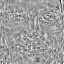
\includegraphics[width=2cm]{395.jpg}
	\end{minipage}
	\begin{minipage}{2cm}
		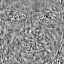
\includegraphics[width=2cm]{396.jpg}
	\end{minipage}
	
	\caption{Porównanie eigenfaces.}
Górny wiersz - wektory 0-4, dolny wiersz - wektory 392-396.
	\label{fig:eigenfaces}
\end{figure}


\subsubsection{Zakłócenia}

\begin{figure}
\centering
		\begin{minipage}{3cm}
			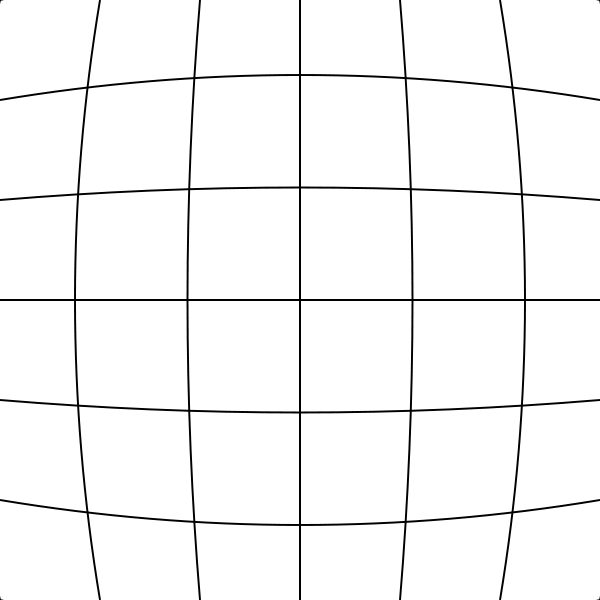
\includegraphics[width=3cm]{600px-Barrel_distortion.png}
		\end{minipage}
		\begin{minipage}{3cm}
			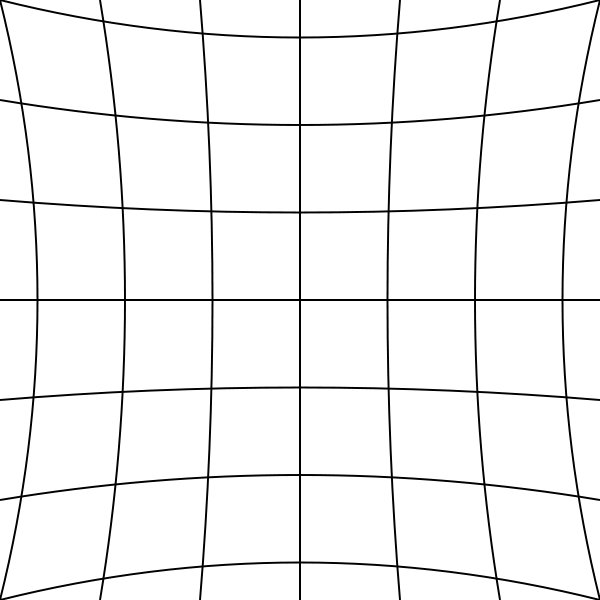
\includegraphics[width=3cm]{600px-Pincushion_distortion.png}
		\end{minipage}
		\begin{minipage}{3cm}
			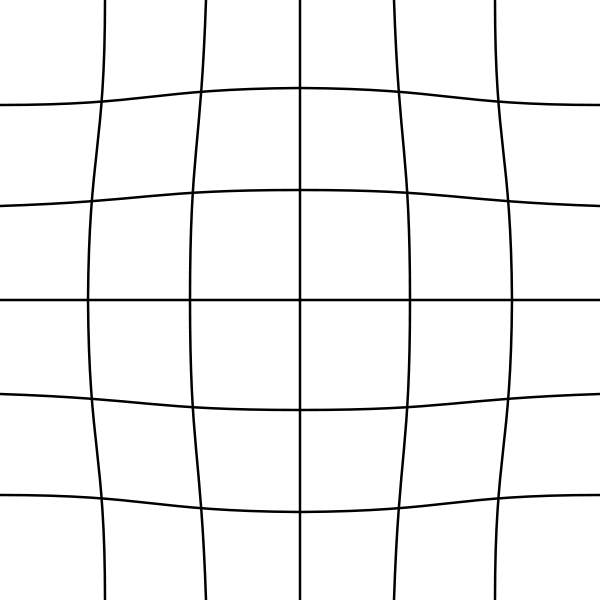
\includegraphics[width=3cm]{600px-Mustache_distortion.png}
		\end{minipage}
	\caption{Różne rodzaje dystorcji (od lewej): beczkowa, poduszkowa oraz falista.}
źródło: https://en.wikipedia.org/wiki/Distortion\_\%28optics\%29
	\label{fig:distortion}
\end{figure}

Zaprezentowany wcześniej model zakłóca brak zakłóceń przy procesie przetwarzania obrazu. W kamerach występują różne rodzaje dystorsji. W dystorsji nie linie proste zostają zniekształcone. Wynika z fizycznej niedoskonałości układów optycznych. Im dalej od osi optycznej tym większe zniekształcenie.

W bibliotece OpenCV przewiduje się współczynniki radialne $k_1, ..., k_6$ oraz styczne $p_1$ i $p_2$. Współczynniki te są wykorzystywane w poprzednim modelu w następujący sposób (podawane za dokumentacją OpenCV \cite{Dokumentacja OpenCV}):
\begin{gather*}
	x' = \frac{x}{z} \\
	y' = \frac{y}{z} \\
	x'' = x' \frac{1+k_1 r^2 + k_2 r^4 + k_3 r^6}{1+k_4 r^2+k_5 r^4+k_6 r^6} +
	2 p_1 x' y' + p_2(r^2 + 2 x'^2)	\\
	y'' = y' \frac{1+k_1 r^2 + k_2 r^4 + k_3 r^6}{1+k_4 r^2+k_5 r^4+k_6 r^6} +
	p_1(r^2 + 2 y'^2) + 2 p_2 x' y'
\end{gather*}


\subsection{Kalibracja kamery}

Kalibracja kamery odbywa się poprzez fotografowanie szachownicy pod różnymi kątami. Następnie zdjęcia są konwertowane do skali szarości i wykrywane są narożniki szachownicy. Pierwsze oszacowanie położenia narożników nie jest dokładne. Estymacja jest poprawiana z wykorzystaniem prostego faktu odnośnie gradientu:

\begin{figure}
\centering
	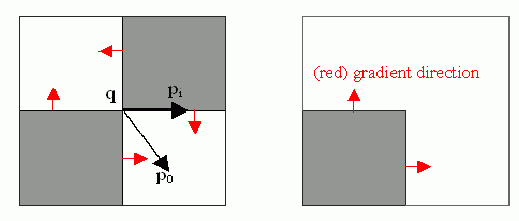
\includegraphics[width=0.70\textwidth]{cornersubpix.png}\par\vspace{1cm}
\caption{Gradient szachownicy. \\ źródło: https://docs.opencv.org/2.4/modules/imgproc/doc/feature\_detection.html}
	\label{fig:gradient}
\end{figure}

Załóżmy że $\bb{q}$ jest narożnikiem szachownicy, a $\bb{p}_i$ jest punktem w bliskim sąsiedztwie. Przyjmijmy wartość błędu daną następującym równaniem:

\begin{equation}
	E_i = \nabla f_{\bb{p}_i}^T (\bb{q} - \bb{p}_i)
\end{equation}

Gdzie $\nabla f_{\bb{p}_i}$ jest gradientem, w punkcie $p_i$. Jest to równanie na iloczn skalarny i będzie ono równe zero, gdy $\bb{p}_i$ będzie prostopadłe do gradientu. Przyrównując powyższe równanie do zera, oraz mnożąc obie strony przez $\nabla f_{\bb{p}_i}$ otrzymujemy:

\begin{align*}
	\nabla f_{\bb{p}_i} \nabla f_{\bb{p}_i}^T \bb{q} - \nabla f_{\bb{p}_i} \nabla f_{\bb{p}_i}^T \bb{p}_i = 0
\end{align*}

W konsekwencji otrzymujemy:

\begin{align}
	\bb{q} = (\nabla f_{\bb{p}_i} \nabla f_{\bb{p}_i}^T)^{-1} \nabla f_{\bb{p}_i} \nabla f_{\bb{p}_i}^T \bb{p}_i
\end{align}

Operacja ta jest powtarzana, aż punkt $q$ uzyska stabilną wartość (jego współrzędne nie będą się zmieniać o większą wartość niż przyjęty próg).

\begin{figure}
\centering
		\begin{minipage}{3.5cm}
			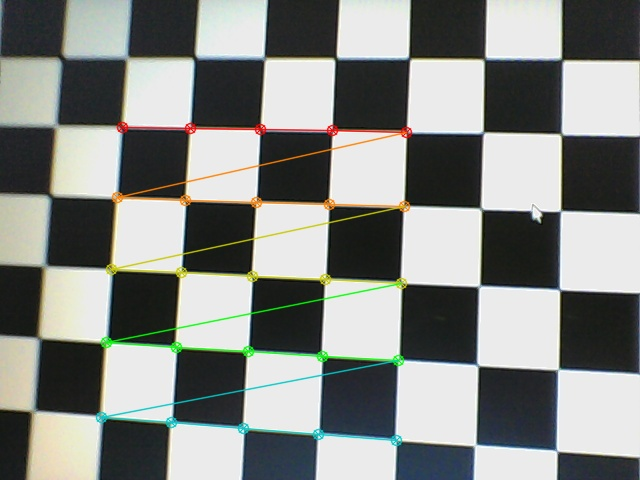
\includegraphics[width=3.5cm]{left1.jpg}
		\end{minipage}
		\begin{minipage}{3.5cm}
			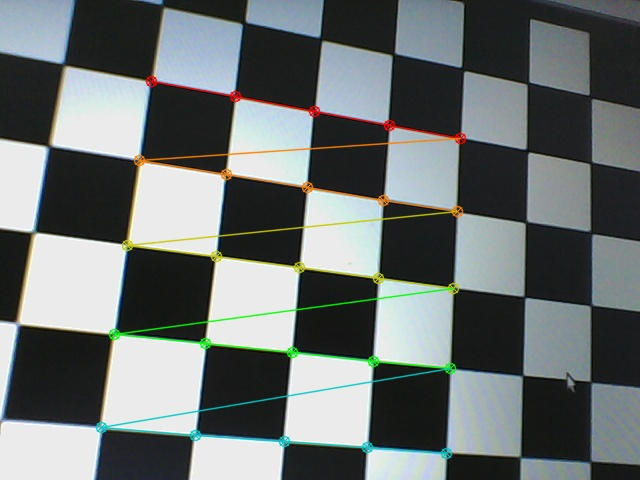
\includegraphics[width=3.5cm]{left10.jpg}
		\end{minipage}
		\begin{minipage}{3.5cm}
			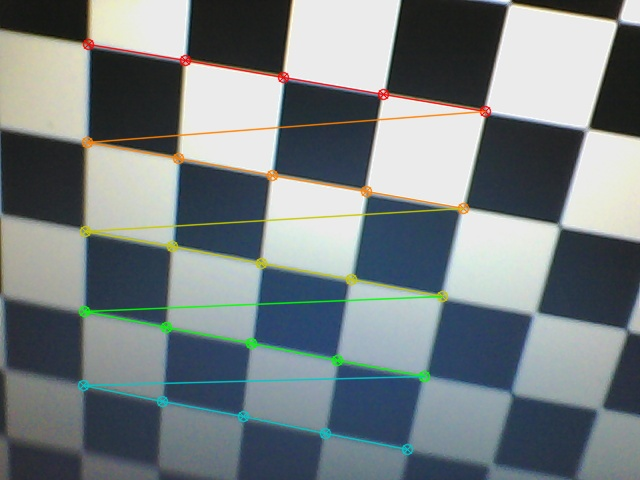
\includegraphics[width=3.5cm]{left27.jpg}
		\end{minipage}
	\caption{Wykryte narożniki szachownicy. }
	\label{fig:corners}
\end{figure}

\begin{figure}
\centering
		\begin{minipage}{3.5cm}
			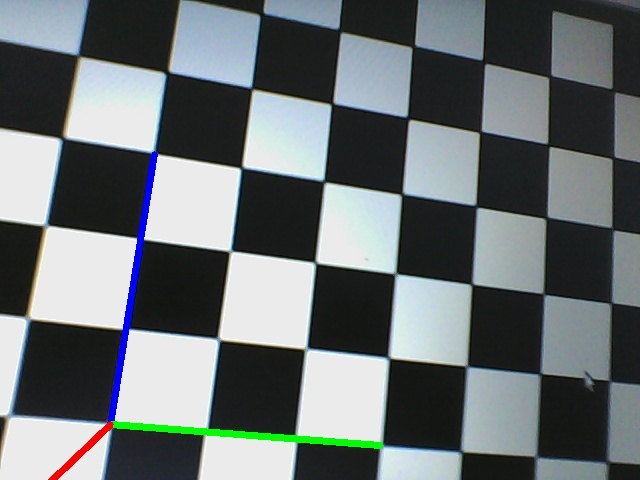
\includegraphics[width=3.5cm]{left8.jpg}
		\end{minipage}
		\begin{minipage}{3.5cm}
			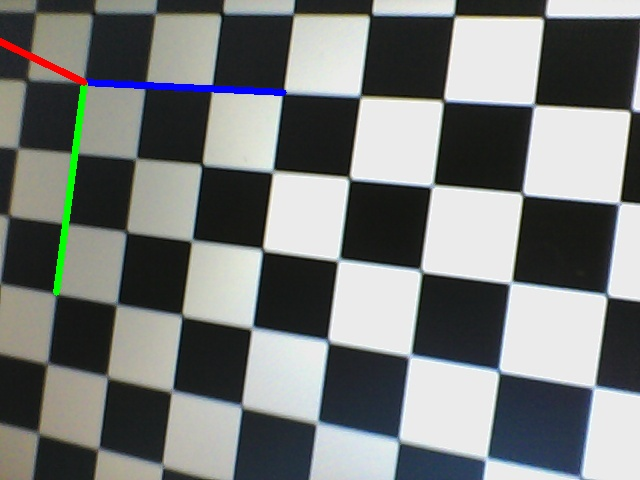
\includegraphics[width=3.5cm]{left17.jpg}
		\end{minipage}
		\begin{minipage}{3.5cm}
			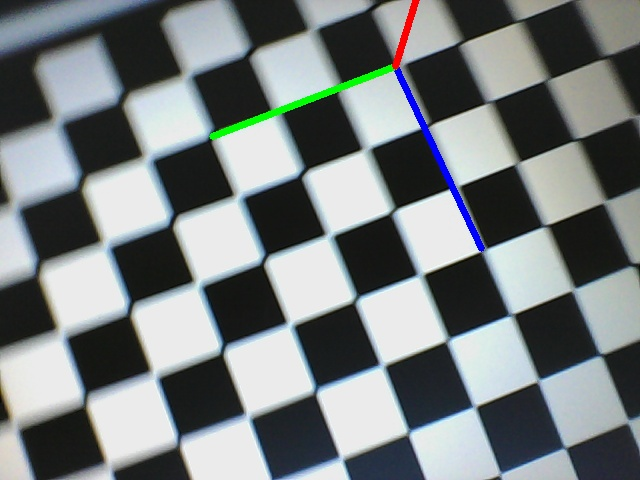
\includegraphics[width=3.5cm]{left24.jpg}
		\end{minipage}
	\caption{Estymacja orientacji szachownicy. }
	\label{fig:pose}
\end{figure}

Dzięki wyznaczonym narożnikom można wyznaczyć wenętrzne i zewnętrzne kamery. Wartości te są następnie wykorzystane do estymacji pozycji \ref{fig:pose}, oraz do usunięcia zakłóceń z obrazu. 

\subsection{Geometria epipolarna}

Zakładając wcześniej przyjęty model rzeczywistej kamery oraz stosując uproszczenie polegające na przeniesieniu płaszczyzny obrazu przed ognisko (w rzeczywistych kamerach płaszczyzna ta znajduje się za ogniskiem) możemy zauważyć pewne zależności geometryczne dla punktu widzianego z dwóch kamer. 

\begin{figure}
\centering
	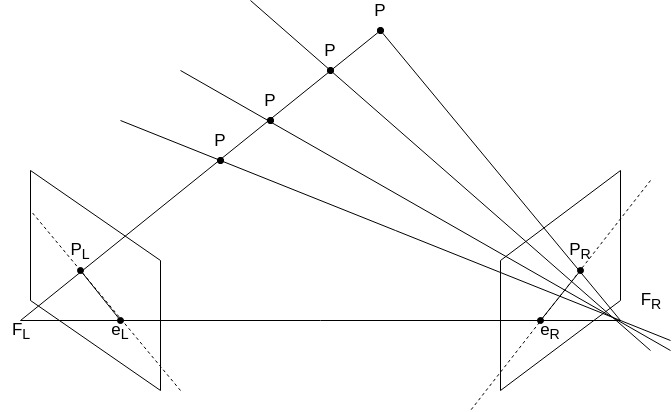
\includegraphics[width=0.70\textwidth]{epipolar.jpg}\par\vspace{1cm}
\caption{Podstawowa koncepcja geometrii epipolarnej.}
	\label{fig:gradient}
\end{figure}

Pierwszym spostrzeniem jest fakt że ogniska obu kamer, punkt P oraz jego projekcje na płaszczyznę obrazu leżą na jednej płaszczyźnie. Linia poprowadzona pomiędzy ogniskami kamer jest nazywana linią główną (ang. baseline). 
Punkty przecięcia linii głównej z płaszczyzną główną ($e$) nazywane są epipolami (ang. epipoles). Jeśli obie kamery się widzą to epipole są widoczne jako środek drugiej kamery na obrazie.
Płaszczyzna przechodząca przez dowolny punkt P widziany w obu kamerach, oraz przez linię główną jest nazywana płaszczyzną epipolarną.
Linia epipolarną nazywamy linię będącą na przecięciu płaszczyzny obrazu z płaszczyzną epipolarną. Wszystkie linie epipolarne przecinają się w epipolach.

Warto zwrócić uwagę na to że linia $F P$ jest widziana na drugim obrazie jako odpowiadająca linia epipolarna. Oznacza to więc, że szukając odpowiednika piksela z jednego obrazu na drugim, należy szukać wzdłuż epilinii, a nie na całym obrazie. Jest to znaczące ułatwienie, które będzie miało duże znaczenie przy obliczaniu dysparycji.

\subsection{Szacowanie głębokości}

Kolejnym krokiem jest obliczenie mapy dysparycji oraz na jej podstawie wyznaczenie głębokości. 

\begin{figure}
	\centering
	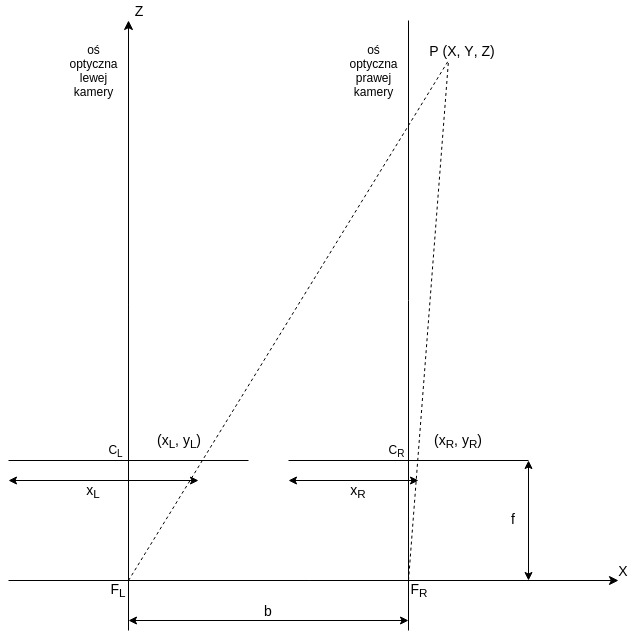
\includegraphics[width=9.5cm]{ekstrakcja.jpg}
	\caption{Ekstrakcja głębi na podstawie dysparycji obrazów z dwóch kamer. }
	\label{fig:extraction}
\end{figure}

Przy ekstrakcji głęgokości jest wykorzystywane podobieństwo trójkątów $P F_L F_R$ oraz $P C_L C_R$ z rys. \ref{fig:extraction}:

\begin{equation}
	\frac{b}{Z} = \frac{b-x_L+x_R}{Z-f}
	\label{eq:disp}
\end{equation}

Po przekształceniach otrzymujemy:

\begin{equation}
	Z = \frac{bf}{x_L-x_R} = \frac{bf}{d}
\end{equation}

Gdzie $d$ jest dysparycją - różnicą wartości odpowiadających sobie pikseli na dwóch obrazach, szukanych wzdłuż epilinii.
Znając ogniskową, odległość między kamerami, oraz obliczając różnicę między analogicznymi pikselami z dwóch obrazów możemy szacować głębię.

Warto zwrócić uwagę że wzór \ref{eq:disp} nie traci na ogólności, gdy punkt $P$ znajdzie się pomiędzy osiami optycznymi kamer, ponieważ do odbliczenia podstawy trójkąta $P C_L C_R$ zostanie wykorzystana odległość między punktem w którym wiązka światła pada na prawą matrycą a osią optyczną prawej kamery. Odlgołość ta może zostać w takim wypadku wyrażona jako $\frac{1}{2}l-x_R$, gdzie $l$ to długość ekranu światłoczułego. Po podstawieniu podobniej wartości za odległość od osi optycznej lewej kamery do punktu przeciącia wiązki światła z lewą matrycą $\frac{1}{2}l$ się uprości i zostaniemy ze wzorem \ref{eq:disp}.

\begin{figure}
	\centering
	\begin{minipage}{5.5cm}
		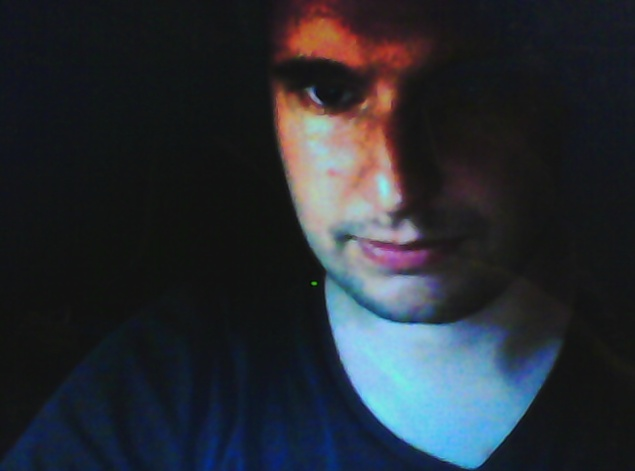
\includegraphics[width=5.5cm]{falt_test_face1L.jpg}
	\end{minipage}
	\begin{minipage}{5.5cm}
		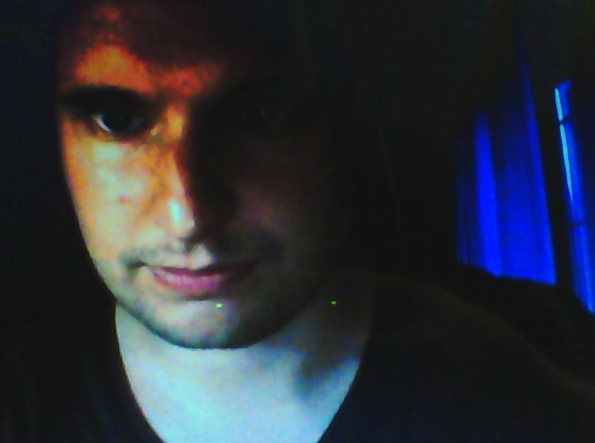
\includegraphics[width=5.5cm]{falt_test_face1R.jpg}
	\end{minipage}
	
	\centerline{
	\begin{minipage}{10.5cm}
		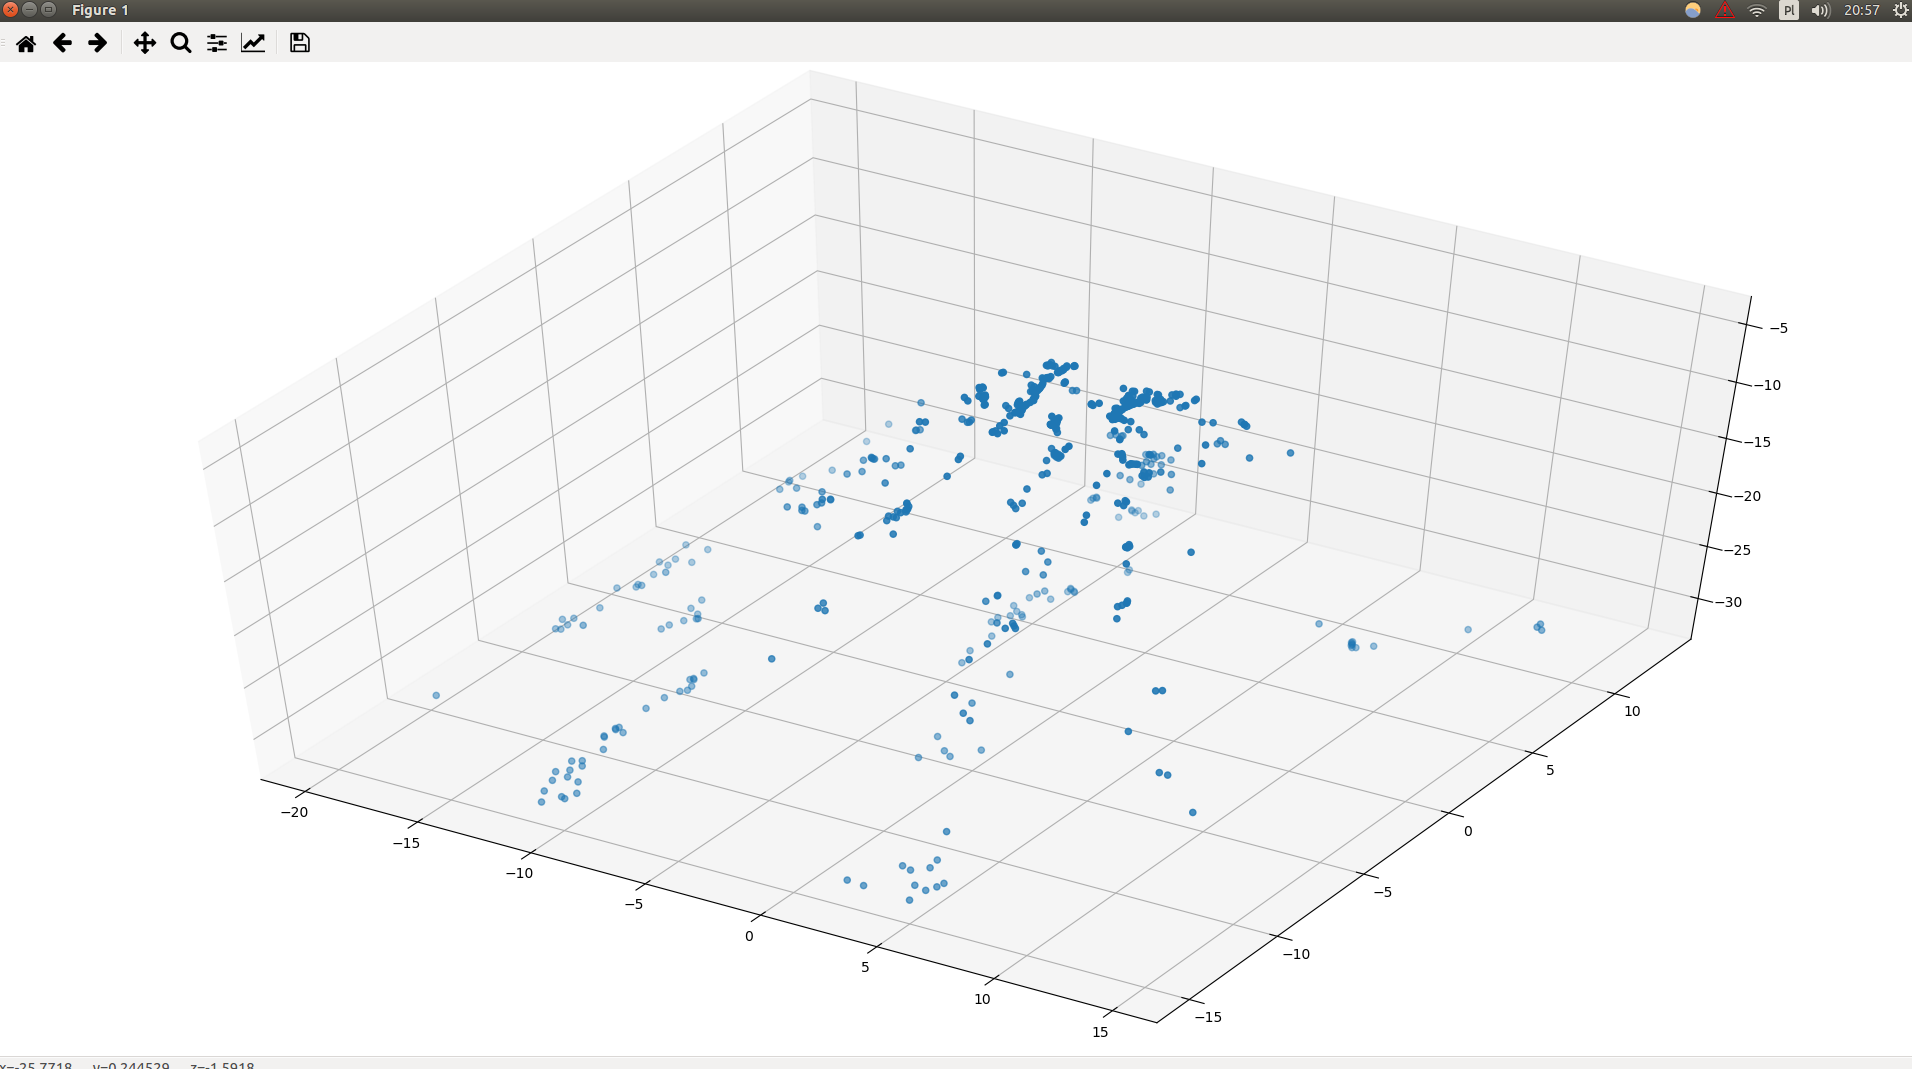
\includegraphics[width=10.5cm]{result_fail.png}
	\end{minipage}}	
	\caption{Obraz płaskiego zdjęcią sfotografowany lewą i prawą kamerą oraz wynik ekstrakcji głebokości. }
	\label{fig:extraction_fail}
\end{figure}


\section{Wyniki}
Dokonano kalibracji kamery, wyznaczno współczynniki wewnętrzne i zewnętrzne kamery. Jednkże nie udało się uzyskać zadowalających rezultatów. Po przedstawieniu systemowi zdjęcia osoby wyświetlonego na laptopie uzyskano mapę głębi przedstawioną na rys. \ref{fig:extraction_fail}. Jak można z łatwością zauważyć zauważyć na mapie głebości otrzymano punkty o różnej głębokości.

Trudno jest określić jedną przyczynę niepowodzenia. Na pewno ważną rolę odgrywa kalibracja kamer. Wielokrotnie podejmowano próbę poprawiania uzyskiwanych wyników poprzez ponowną kalibrację, ale nie wpłynęło to w znaczący sposób na rezultaty. W związku z ograniczoną ilością czasu projekt nie mógł zostać ukończony, pomimo wielu godzin poświęconych na analizę problemu.

\chapter{Zakończenie}



\newpage
\begin{thebibliography}{9}

\bibitem{Pattern recognition}
Christopher M. Bishop.
\textit{Pattern recognition and machine learning}.
Springer Science + Business Media, New York 2009

\bibitem{Ślot}
Krzysztof Ślot.
\textit{Rozpoznawanie biometryczne. Nowe metody ilościowej reprezentacji obiektów}
Wydawnictwo Komunikacji i Łączności, Warszawa 2000

\bibitem{Osowski}
Stanisław Osowski.
\textit{Sieci Neuronowe w ujęciu algorytmicznym}
Wydawnictwo Naukowo-Techniczne, Warszawa 1996

\bibitem{AdaBoost}
Yoav Freund, Robert E. Schapire.
\textit{A Short Introduction to Boosting}
AT\&T Labs - Research. Shannon Laboratory

\bibitem{Kaskada Haara}
Paul Viola, Michael Jones.
\textit{Rapid Object Detection using a Boosted Cascade of Simple Features}.
Cambridge 2001

\bibitem{Landmark face detector}
Vahid Kazemi and Josephine Sullivan
\textit{One Millisecond Face Alignment with an Ensemble of Regression Trees}
KTH, Royal Institute of Technology
Computer Vision and Active Perception Lab, 2014

\bibitem{Stereo}
Hartley, R.~I. i Zisserman, A.
\textit{Multiple View Geometry in Computer Vision}
Cambridge University Press, 2004

\bibitem{OpenCV}
Itseez.
\textit{Open Source Computer Vision Library}
\\\texttt{https://github.com/itseez/opencv}

\bibitem{Dokumentacja OpenCV}
Dokumentacja biblioteki OpenCv 
\\\texttt{https://docs.opencv.org/2.4/index.html}

\bibitem{Tutoriale OpenCV}
Zbiór tutoriali z OpenCV
\\\texttt{https://docs.opencv.org/3.0-beta/doc/py\_tutorials/py\_tutorials.html}

\bibitem{scikit-learn}
Pedregosa, F. and Varoquaux, G. and Gramfort, A. and Michel, V.
         and Thirion, B. and Grisel, O. and Blondel, M. and Prettenhofer, P.
         and Weiss, R. and Dubourg, V. and Vanderplas, J. and Passos, A. and
         Cournapeau, D. and Brucher, M. and Perrot, M. and Duchesnay, E.
 \textit{Scikit-learn: Machine Learning in {P}ython}
 Journal of Machine Learning Research, volume 12, pages 2825-2830, year 2011

\bibitem{FaceID hacked}
News o pokonaniu zabezpieczeń systemu FaceID
\\\texttt{http://www.bkav.com/d/top\-news/\-/view\_content/content/103968/face\-id\-beaten\-by\-mask\-not\-an\-effective\-security\-measure}

\end{thebibliography}

\tableofcontents

\listoffigures

\end{document}